\section{Anti aliasing filter}
\subsection{Formål}
Analog til digital konverteren sampler ved en vis frekvens. Det er derfor vigtigt, ifølge Nyquist’s sætning, at begrænse indgangssignalet til halvdelen af denne samplingsfrekvens. Dette udelukker støj ved højere frekvenser.\\

Dette kan realiseres ved hjælp af et anti aliasing filter (herefter AA filter). Samplingsfrekvensen af sat til 44.1kHz, det vil derfor være ideelt at påføre et AA filter med en betydelig dæmpning ved 22.5kHz.\\
\subsection{Overvejelser}
Når der arbejdes med lydsignaler er det vigtigt at overveje gruppeløbetiden. Denne beskriver hvor stor en forsinkelse forskellige frekvenser har i forhold til gengivelsen. Ud fra dette blev der indledningsvis valgt et bessel filter, da denne type filter har en konstant gruppeløbetid op til knækfrekvensen. Senere på forløbet blev afklaret at forsinkelsen skulle ligge i millisekund før det var tydelig hørbart. Der blev derfor taget en beslutning om at skifte til Butterworth filtre, da disse har en stejlere dæmpnings hældning og kræver færre komponenter.\\
\subsection{Parametre, udregning og Sallen Key}
Butterworth filteret blev valgt som det endelige filter. 
Det vælges at knækfrekvensen skal ligge ved 17kHz med en dæmpning på -3dB. Ved hjælp af Matlab (der refereres til bilag \ref{void}) udregnes at amplituden ved 22.5kHz kan dæmpes med -12dB med at 5. ordens butterworth filter.\\
Der ønskes tre overføringsfunktioner på formen\\
\begin{center}
	$H(s) = \dfrac{1}{s^2+b_1\cdot s + b_0}$\\
\end{center}
Ved hjælp af tablerne \ref{void} i bilag, kan overføringsfunktionerne for de tre aktive filtre findes.

\begin{figure}
	
\begin{center}
	\begin{itemize}	
 $H_1(s) = \dfrac{1}{s+1}$ \\ 
 $H_2(s) = \dfrac{1}{s^2 + 0.618034\cdot s + 1}$\\
 $H_3(s) = \dfrac{1}{s^2 + 1.618034\cdot s + 1}$\\

	\end{itemize}
\end{center}
\end{figure}

Den totale overføringsfunktion kan findes via tabel \ref{void}.\\ 
\begin{center}
 $H(s) = \dfrac{1}{s^5+3.236068\cdot s^4 + 5.236068\cdot s^3 + 5.236068\cdot s^2 + 3.236068\cdot s +1}$
\end{center}
\subsection{Realisering}
Et 5. ordens filter kan realiseres aktivt ved at kaskadekoble et 1. ordens filter med to 2. ordens filtre som vist på figur  \ref{fig::filter_kask_butterworth}. Ved realisering af det aktive filter benyttes Sallen-Key, en filter topologi der anvendes til at realisere 2. ordens aktive filtre. 
\begin{figure}[h!]
	\centering
	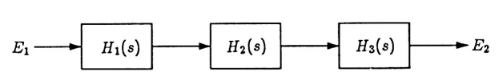
\includegraphics[scale=0.7]{./billeder/Kaskade.png}
	\caption{Kaskade af flere butterworth filtre.}
	\label{fig::kask_butterworth}
\end{figure}
\FloatBlock
Stage 1 er et 1. ordens butterworth filter. Der designes ud fra formlen:\\
\begin{center}
	$f_c = \dfrac{1}{2\cdot\pi\cdot R C}$\\
\end{center} 	
hvor $f_c$ er knækfrekvensen sat ved $17kHz$.
R1 vælges til $10K\Omega$ og C1 udregnes til $936pF$.\\
\begin{figure}[h!]
	\centering
	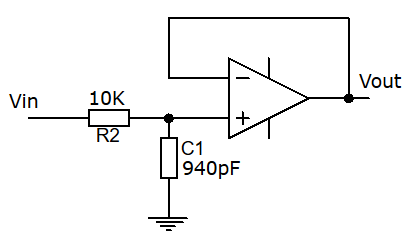
\includegraphics[scale=0.3]{./billeder/stage1}
	\caption{Stage 1 filter opbygning.}
	\label{fig::stage1}
\end{figure}
\FloatBlock
Stage 2 designes ved hjælp af formlen\\
\begin{center}
\begin{math}
H(s) = \dfrac{1}{1+C1(R1+R2)\cdot s+C1C2R1R2\cdot s^2}
\label{eq::SallenKey}
\end{math}
	
\end{center} 

Her sættes $C2(R1+R2) = \dfrac{1}{w_0\cdot Q}$ og $C1C2R1R2 = \dfrac{1}{w_0^2}$, hvor $Q = \dfrac{\sqrt{b_0}}{b_1}$ og $w_0 = 2 \pi  f_c$.
\\R1 og R2 vælges til $32K\Omega$. Ud fra to ligninger med to ubekendte, udregnes C1 til at være $90pF$, og C2 udregnes til $936pF$.\\
Ud fra formel \ref{eq::SallenKey} udregnes også stage 3. Her vælges R2 til at være $155k\Omega$ og C2 til at være $936pF$, C1 udregnes til at være $93pF$ og R1 til $6.4K\Omega$. 
\begin{figure}[h!]
	\centering
	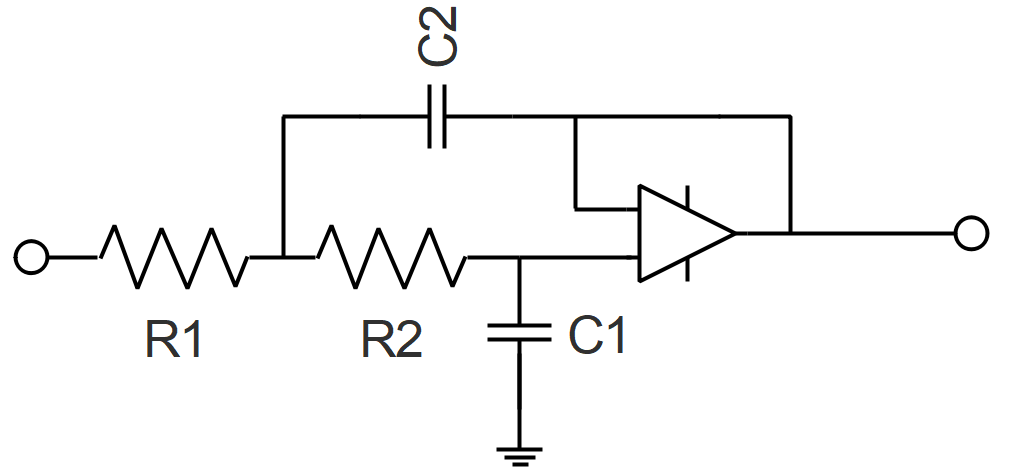
\includegraphics[scale=0.3]{./billeder/stage23}
	\caption{Stage 2 og 3 filter opbygning.}
	\label{fig::filter_stage2}
\end{figure}
\FloatBlock
\subsection{Simulering}
Simuleringen af AA filteret er udført med LTspice. Som det ses på figur \ref{fig::aa_sim}, findes en dæmpning på -3dB ved 17kHz og en dæmpning på -12dB ved 22.5kHz. Forskellen i gruppeløbetiden er maksimalt $18 \mu s$.
\begin{figure}[h!]
	\centering
	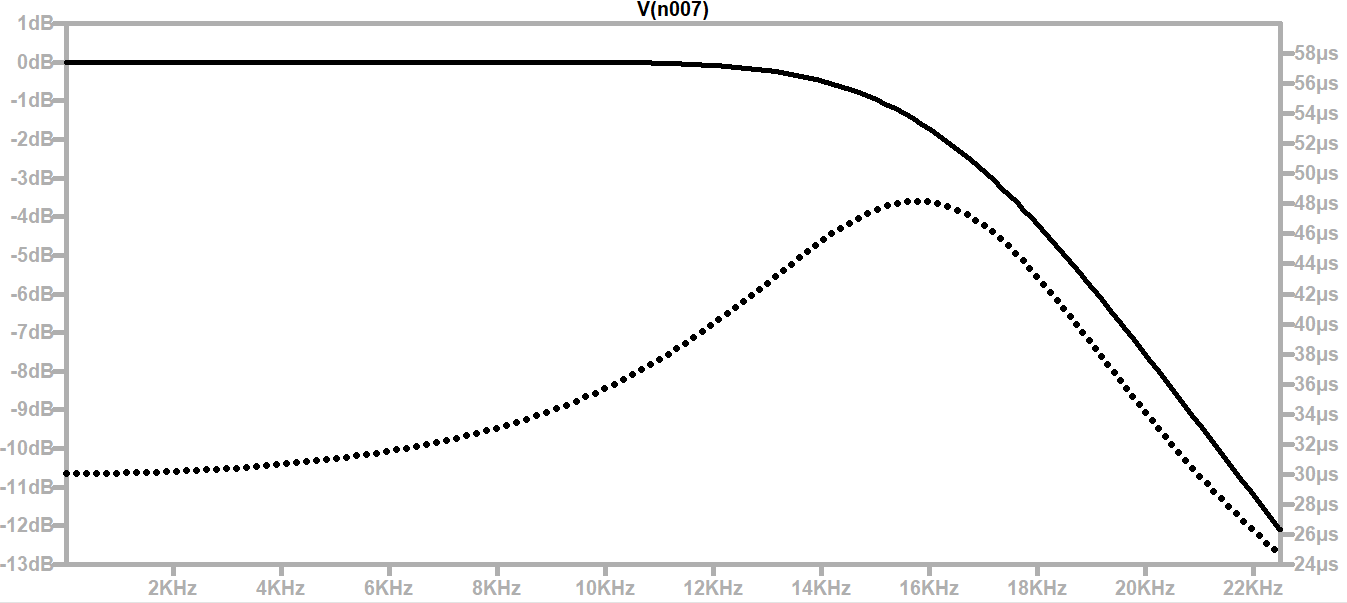
\includegraphics[scale=0.2]{./billeder/aa_sim1}
	\caption{Simulering af AA filteret. Sort: Amplitude, Grå: Gruppeløbetid.}
	\label{fig::afilter_aasim}
\end{figure}
\FloatBlock
Denne kaskade af filtre vil generere 5 poler. En reel pol i stage 1, to komplekse poler i stage 2 og to komplekse poler i stage 3. Disse kan ses i figur \ref{void}.

\begin{figure}[h!]
	\centering
	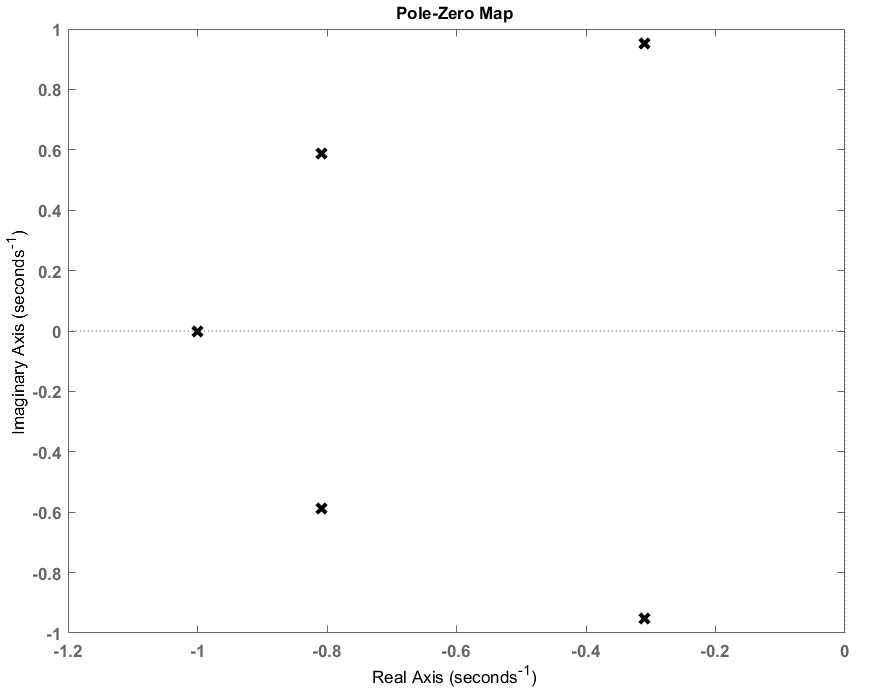
\includegraphics[scale = 0.4]{./billeder/pzmap}
	\caption{Kortlægning af polerne i AA og rekonstruktions filterne.}
	\label{fig:afilter_pol}
\end{figure}
\FloatBlock
\section{Rekonstruktions filter}
\subsection{Formål}
I et system med både analog og digitale signaler, bruges et rekonstruktions filter (eller anti image filter) til at genererer et glat analog signal fra udgangssignalet fra bla. en DAC. Et digitalt lyd signal har en trappetrin type bølgeform som indeholder en del højfrekvent energi kaldet "images". Et rekonstruktions filter konstruerer en mere jævn version af det originale signal.
\subsection{Parametre og udregning}
Det er almindelig praksis at benytte et filter til rekonstruktion, magen til det filter der anvendes til antialiasing. For udregninger af dette filter, henvises til afsnit \ref{void}.
\subsection{Test og målinger}